\documentclass[11pt]{article}

\usepackage{times}
\usepackage[utf8]{inputenc} % allow utf-8 input
\usepackage[T1]{fontenc}    % use 8-bit T1 fonts
\usepackage{url}            % simple URL typesetting
\usepackage{graphics}
\usepackage{color}
\usepackage{amsfonts}       % blackboard math symbols
\usepackage{amsmath}       % blackboard math symbols
\usepackage{amssymb}
\usepackage{booktabs}
\usepackage{array}

\usepackage{lipsum}

\usepackage{tikz}
\usetikzlibrary{angles,quotes,calc}

\usepackage{geometry}
\geometry{left=2.8cm,right=2.8cm,top=2.6cm,bottom=2.6cm}
\usepackage{fancyhdr}
\pagestyle{fancy}
\usepackage{hyperref}% should be the last package you include

\newcommand{\theteam}{}
\newcommand{\team}[1]{\def\theteam{#1}}


\fancyhead[L]{\theteam}
\fancyhead[R]{\thepage}
\cfoot{}

\setlength{\parindent}{0pt}

\team{WayneGradientzky: Rajinish Aneel Bhatia, Bartol Markovinović, Mohd Khizir Siddiqui}
\title{RL-Course 2025/26: Final Project Report}
\author{\theteam}

\begin{document}
\maketitle

\section{Introduction}\label{sec:intro}
% TODO::: NOT SURE WHY THIS SECTION IS MESSING UP THE PLOTS?????
% The report presents the implementation of three reinforcement learning algorithms by the \emph{WayneGradientzky} team.
% The algorithms were finally evaluated on the Hockey competition hosted by the Martius Lab.
% \texttt{Hockey} is a 2D-multi-agent, fully observable environment where two agents compete to score goals by hitting a puck into the opponent's goal.

% The algorithms implemented are as follows:
% \begin{itemize}
%     \item \textbf{Task-Driven Model Predictive Control (TDMPC)} by Bartol Markovinović
%     \item \textbf{Twin Delayed Deep Deterministic Policy Gradient (TD3)} \cite{fujimoto2018:TD3} by Rajinish Aneel Bhatia
%     \item \textbf{Soft Actor-Critic (SAC)} \cite{HaarnojaAbbeelLevine2018:SAC} by Mohd Khizir Siddiqui
% \end{itemize}

% All the implementations are available on the GitHub repository \url{https://github.com/BartolMarko/HockeyRL}.

\section{Temporal Difference Learning for Model Predictive Control (TD-MPC)}

Temporal Difference Learning for Model Predictive Control (TD-MPC)~\cite{TDMPCv1} is a continuous action space model-based RL algorithm that combines learning a Task-Oriented Latent Dynamics (TOLD) model with trajectory optimization using a variation of the Model Predictive Path Integral (MPPI) method. The TOLD model consists of the following learned components:

\begin{itemize}
    \item \textbf{Latent Encoder}: $z_t = h_\theta(s_t)$ -- Encodes the state into a latent representation which captures relevant features for predicting rewards, dynamics, and value.
    \item \textbf{Latent Dynamics}: $z_{t+1} = d_\theta(z_t, a_t)$ -- Predicts the next latent state given the current latent state and agent's action. This allows the model to roll out trajectories during planning. For hockey environment, dynamics model also implicitly predicts opponent's behavior since the opponent's features are part of the state and opponent's actions affect the next state.
    \item \textbf{Reward}: $\hat{r_t} = r_\theta(z_t, a_t)$ -- Predicts immediate reward for taking an action in a given latent state.
    \item \textbf{Q-Value Function}: $\hat{Q_t} = Q_\theta(z_t, a_t)$ -- Predicts the value of taking an action in a given latent state. Two Q-networks are used to mitigate overestimation bias, similar to TD3.
    \item \textbf{Policy}: $\hat{a_t} \sim \pi_\theta(z_t)$ -- Outputs a distribution over actions given the latent state. Policy is used for training the Q-value function and for generating additional trajectories during planning.
\end{itemize}

Models $h_\theta, d_\theta, r_\theta, Q_\theta$ are jointly trained by minimizing the loss
$
\mathcal{J}(\theta, \Gamma) = \sum_{i=t}^{t+H} \lambda^{i-t} \mathcal{L}(\theta, \Gamma_i)
$
where the objective $\mathcal{L}(\theta, \Gamma_i)$ for each step $i$ consists of reward prediction error, value loss with respect to the TD target, and L2 loss between the predicted next latent state and the encoded actual next state:
$$
\mathcal{L}(\theta, \Gamma_i) = 
c_1 \| r_\theta(z_i, a_i) - r_i \|_2^2 + 
c_2 \| Q_\theta(z_i, a_i) - (r_i + \gamma Q_{\theta'}(z_{i+1}, \pi_{\theta}(z_{i+1}))) \|^2 + 
c_3 \| d_\theta(z_i, a_i) - h_{\theta'}(s_{i+1}) \|_2^2
$$

Symbol $\Gamma$ denotes a trajectory of states, rewards and agent's actions sampled from the replay buffer, $\lambda$ is a constant that decreases importance of losses for later steps, $\gamma$ is the discount factor, and $c_1$, $c_2$, $c_3$ are constants that balance the different loss components. For the Q-value loss and the latent dynamics loss, the target networks $\theta'$ are used. Target networks are updated every 2 mini-batch updates with slow-moving averages of the main network parameters to stabilize training. For sampling mini-batches of trajectories, a prioritized experience replay buffer is used, where states are sampled with probability proportional to their TD error. The policy network is trained separately, by minimizing the temporally weighed Q-value objective of the same sampled trajectories: 
$\mathcal{J}_\pi(\theta) = - \sum_{i=t}^{t+H} \lambda^{i-t} Q_{\theta}(z_i, \pi_\theta(z_i))$.

To select an action, several iterations of modified MPPI planning are performed. In the first iteration, $N$ random action sequences of length $H$ (horizon) are sampled from the normal distribution $\mathcal{N(\mu, \sigma)}$ and rolled out using the learned dynamics model to obtain future latent states and rewards $H$ steps into the future. Additionally, the policy network is used to generate extra trajectories by rolling out the policy model and adding truncated Gaussian noise.
Each trajectory is scored by the discounted sum of predicted rewards and the final Q-value. The top $K$ trajectories are selected and weighed by their exponentiated scores to update $\mu$ and $\sigma$ for the next iteration. After last iteration, a trajectory is sampled from the score weighed multinomial distribution of the final elite set and the first action of that trajectory is executed.

\subsection{Network Architecture Changes}

Initially, each part of the TOLD model was implemented as an MLP with ELU function~\cite{ELU} as the non-linearity, as described in the original paper.
However, this resulted in training instability caused by exploding loss values. To solve this issue, network architectures described in the TD-MPC2 paper~\cite{TDMPCv2} were implemented. Activation function was changed to Mish~\cite{Mish}, Layer Normalization was added, and latent space was normalized with SimNorm~\cite{TDMPCv2}. Furthermore, the Q-value and reward networks were changed to output logits of a softmax distribution over exponentially spaced bins, as described in DreamerV3~\cite{DreamerV3}.

\subsection{Adding Ideas from iCEM to the Planning Algorithm}

One attempt to improve the planning part of TD-MPC was to implement ideas from the Improved Cross-Entropy Method (iCEM)~\cite{iCEM}. These included sampling actions from temporally correlated colored noise instead of independent Gaussian noise, keeping a fraction of the elite set between iterations, including the shifted elite set from previous step into the initial trajectory set of the next iteration, and executing the best action from the final elite set instead of sampling from the score weighted distribution.

\subsection{Action Hints -- Guiding Planning with Custom Action Sequences}

Another idea to improve planning was to replace a part of the initial random action sequences with hand-crafted action sequences that either lead agent to a future position of the puck or to one of the equidistantly spaced positions in front of the goal. These action sequences were generated with PD control, and the idea was used in conjunction with keeping a fraction of the elite set between planning iterations to potentially preserve exact trajectories that lead to the puck or the goal.

\begin{figure}[h]
    \centering
    \begin{minipage}{0.4\textwidth}
        \centering
        \includegraphics[width=\textwidth]{tdmpc_images/action_hints.png}
        \caption{Illustration of action hints}
        \label{fig:action_hints}
    \end{minipage}
    \hfill
    \begin{minipage}{0.4\textwidth}
        \centering
        \includegraphics[width=\textwidth]{tdmpc_images/mirror.png}
        \caption{State and action mirroring}
        \label{fig:mirror}
    \end{minipage}
\end{figure}

\subsection{Training Setup and Self-Play}

For training, only the terminal (sparse) reward of $+10$ for winning and $-10$ for losing was used. When adding an episode to the replay buffer, the mirrored episode with respect to the horizontal axis (\ref{fig:mirror}) was also added. This doubles the amount of training data and encourages model to learn symmetric strategies. 

\subsubsection{Training Curriculum}

Training is started against only weak and strong bots, and a frozen checkpoint of the model is added to the opponent pool every 100 000 steps, or earlier if win rate against all opponents exceeds $80\%$. Additionally, 3 TD3 agents with different behaviors are added to the opponent pool after 2 million steps. Maximum opponent pool size is set to 10, and when the pool is full, the oldest frozen checkpoint is removed. This curriculum ensures that the model is exposed to a variety of opponents of appropriate difficulty throughout training.
To monitor generalization performance against unseen strong opponents, model was \textbf{not trained, but only evaluated} against publicly available SAC agent from last year's competition.

\subsubsection{Windowed Thompson Sampling Opponent Selection}

Since all opponents in the training pool are beatable due to the curriculum, selecting the most challenging opponent seems like a reasonable strategy to maximize learning signal. To do this, the number of wins, draws, and losses against each opponent in the pool was tracked in a sliding window of the last 100 games (in total, not per opponent). Then, win, loss and draw rates of the TD-MPC agent against each opponent were estimated by sampling from a Dirichlet distribution with parameters $\alpha = [\text{wins}+1, \text{losses}+1, \text{draws}+1]$. The opponent where the $loss\_rate + 0.5 * draw\_rate$ is maximized is selected. The intuition behind this is that the problem of choosing the most challenging opponent can be seen as similar to a multi-armed bandit problem, where each opponent is an arm and the reward is 1 for a loss, 0.5 for a draw, and 0 for a win. Using only last 100 episodes accounts for constant change of policy, and Dirichlet distribution was chosen because it is a conjugate prior for the multinomial distribution, which models the outcomes of games against each opponent.

\subsection{Experiment Results}

All experiment configurations were first run for 3 million steps (or less if unsuccessful), and the best performing experiments were prolonged to 10 million steps. In Figure \ref{fig:performance} we see that during all experiments the model quickly learns to defeat the weak bot. However, with the initial bad model architecture, the win rate against the weak bot plummets after 500 thousand steps, showing the training instability. After fixing the architecture, the model maintains a high win rate against the weak bot. The variations that used iCEM ideas do not generalize well to the validation agent, regardless of the colored noise $\beta$ parameter. The checkpoint that generalized the best seemed to be the one with action hints trained for 4.3 million steps. This was confirmed with the final tournament results.
Additionally, a number of different smaller modifications were tested, such as training with defensive mode, using closeness to goal as an additional reward signal, and using dropout in Q-value networks, but they did not lead to any improvements.

\begin{figure}[h]
    \centering
    \includegraphics[width=0.8\textwidth]{tdmpc_images/performance.png}
    \caption{Evaluation win rates against Weak Bot and the SAC validation agent for different experiments}
    \label{fig:performance}
\end{figure}

\section{Twin Delayed Deep Deterministic Policy Gradient (TD3)}

Twin Delayed Deep Deterministic Policy Gradient (TD3)~\cite{fujimoto2018:TD3} is a 
model-free, off-policy algorithm for continuous action spaces, improving over DDPG via 
clipped double Q-learning, delayed policy updates, and target policy smoothing. TD3 
maintains two Q-networks ($Q_{\phi_1}$ and $Q_{\phi_2}$) and uses their minimum as the 
TD target:
%
\[ y = r + \gamma \min_{i=1,2} Q_{\phi_{i}'}(s', \tilde{a}), \quad
   \tilde{a} = \pi_{\theta'}(s') + \epsilon, \quad 
   \epsilon \sim \texttt{clip}(\mathcal{N}(0,\sigma), -c, c) \]
%
Each critic minimizes the squared Bellman error 
$\mathcal{L}(\phi_i) = \mathbb{E}_{(s,a,r,s')\sim\mathcal{D}}(Q_{\phi_i}(s,a)-y)^2$, 
while the actor maximizes $J(\theta) = \mathbb{E}_{s\sim\mathcal{D}} 
Q_{\phi_1}(s,\pi_\theta(s))$ and is updated every 2 critic steps.

\subsection{Method}
\subsubsection{N-Step Returns}

Instead of the standard one-step TD target, we use $n$-step returns to propagate reward 
signal faster:
%
\[ y = r(s_0) + \gamma r(s_1) + \dots + \gamma^{n-1}r(s_{n-1}) + \gamma^n q(s_n, \tilde{a}) \]

\subsubsection{Custom Opponent and Bank-Shot Reward}

We noticed early on that the model did not always manage to learn ricochet (bank) shots, so to help it defend against opponents that hit those shots we introdued a hard-coded opponent that always plays them.
Given puck position $P$, goal position $G$, and $T$ as the target we must shoot at to reach $G$. Then $T_y$ is known because that is the boundary and we only need to find $T_x$. We can assume that $T_x \ge P_x$ and $G_x \ge T_x$. If we assume frictionless walls than $\theta$ = $\phi$.

\begin{center}
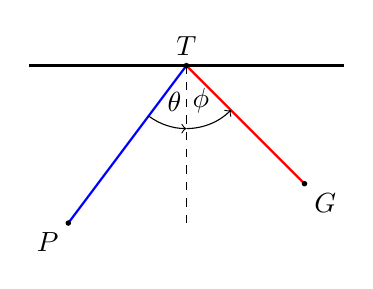
\begin{tikzpicture}[scale=0.5]
  \coordinate (P) at (-3,-2);
  \coordinate (G) at (3,-1);
  \coordinate (T) at (0,2);
  \coordinate (W1) at (-4,2);
  \coordinate (W2) at (4,2);
  \coordinate (N) at (0,-2);
  \draw[thick] (W1) -- (W2);
  \draw[thick, blue] (P) -- (T);
  \draw[thick, red]  (T) -- (G);
  \draw[dashed] (T) -- (N);
  \fill (P) circle (2pt) node[below left]  {$P$};
  \fill (G) circle (2pt) node[below right] {$G$};
  \fill (T) circle (2pt) node[above]       {$T$};
  \pic[draw, ->, angle radius=0.8cm, "$\theta$"]{angle = P--T--N};
  \pic[draw, ->, angle radius=0.8cm, "$\phi$"]  {angle = N--T--G};
\end{tikzpicture}
\end{center}

From $\tan\theta = \tan\phi$ we obtain:
%
\[ T_x = \frac{|T_y - P_y|\,G_x + |T_y - G_y|\,P_x}{|T_y - G_y| + |T_y - P_y|} \]
%
This agent achieves ${\approx}94\%$ win rate against the weak opponent and ${\approx}80\%$ 
against the strong opponent. We also shaped the reward by calculating how aligned the agent's direction was to this direction to encourage the learning agent to prefer shots in this direction.

\subsubsection{Layer Normalization}

\textbf{Layer Normalization.} Layer normalization normalizes activations across the feature dimension for each sample
independently. For a given input vector $x$, it computes:
\[
    \texttt{LayerNorm}(x) = \frac{x - \mu}{\sigma + \varepsilon}\,\gamma + \beta
\]
where $\mu$ and $\sigma$ are the mean and standard deviation of $x$, and $\gamma$,
$\beta$ are learnable scale and shift parameters. In the RL setting this reduces
sensitivity to the scale of inputs and gradients, which can vary
dramatically during training. We apply LayerNorm after each linear layer in both
actor and critic networks.

\subsection{Experiments}

\subsubsection{Training in Phases (Opponent Scheduling)}
Training proceeded in three phases. Phase 1 used only the weak opponent. Phase 2 sampled 
weak/strong opponents with probabilities $30\%$/$70\%$. Phase 3 used a mixed pool: $20\%$ 
weak, $20\%$ strong, $10\%$ custom bank-shot opponent, and $50\%$ from a rolling queue of 
past checkpoints (self-play). 
An adaptive opponent selection strategy based on Thompson sampling was evaluated as an 
alternative but underperformed the manual schedule, as shown in Figure~\ref{fig:thompson}.

\begin{figure}[h]
    \centering
    \begin{minipage}{0.48\textwidth}
        \centering
        \includegraphics[width=\textwidth]{td3_images/baseline1.png}
        \caption{Winrate (trained in phases)}
        \label{fig:baseline}
    \end{minipage}
    \hfill
    \begin{minipage}{0.48\textwidth}
        \centering
        \includegraphics[width=\textwidth]{td3_images/thompson.png}
        \caption{Winrate (trained using Thompson sampling)}
        \label{fig:thompson}
    \end{minipage}
\end{figure}

\subsubsection{Self-Play}
Self play was the part of the third phase of training and was implemented by keeping a queue of $50$ checkpoints and adding a new checkpoint every $50000$ timesteps. This ensured that the model had enough learning experience from each of its previous checkpoints to be able to defeat them.

\subsubsection{N-Step Returns, Episode Mirroring and Environment Scheduling}

$N$-step returns and episode mirroring improve the speed of learning as reflected in
(Figure~\ref{fig:n_steps_result}), compared to
one-step TD targets. We chose 3-step for the final training. Environment scheduling ($30\%$ SHOOTING\_MODE, $70\%$ DEFENSE\_MODE)
was introduced in Phase 3. Figure~\ref{fig:right_possesion_winrate} shows the win rate
when the opponent starts with possession and confirms a clear improvement.

\begin{figure}[h]
    \centering
    \begin{minipage}{0.48\textwidth}
        \centering
        \includegraphics[width=\textwidth]{td3_images/n_step_results.png}
        \caption{Win rate vs.\ past checkpoints ($n$-step returns)}
        \label{fig:n_steps_result}
    \end{minipage}
    \hfill
    \begin{minipage}{0.48\textwidth}
        \centering
        \includegraphics[width=\textwidth]{td3_images/right_possesion_win_rate.png}
        \caption{Win rate when opponent starts with possession using environment scheduler}
        \label{fig:right_possesion_winrate}
    \end{minipage}
\end{figure}

\subsubsection{Bank-Shot Reward}

The bank-shot preference reward visibly shifts puck density toward the walls
(Figures~\ref{fig:normal_reward},~\ref{fig:bank_pref_reward}), confirming that the
agent learned to incorporate ricochet shots into its strategy.

\begin{figure}[h]
    \centering
    \begin{minipage}{0.48\textwidth}
        \centering
        \includegraphics[width=\textwidth]{td3_images/heatmapnormal.png}
        \caption{Puck density — standard reward}
        \label{fig:normal_reward}
    \end{minipage}
    \hfill
    \begin{minipage}{0.48\textwidth}
        \centering
        \includegraphics[width=\textwidth]{td3_images/heatmapbank_pref.png}
        \caption{Puck density — bank-shot preference reward}
        \label{fig:bank_pref_reward}
    \end{minipage}
\end{figure}

\subsubsection{Layer Normalization}

LayerNorm converged faster against the fixed bots (Figure~\ref{fig:bs_v_ln}) but hurt
generalization during self-play: the agent progressively drew against all previous
checkpoints (Figure~\ref{fig:ln_draw_rate}) rather than maintaining dominance, so it
was excluded from the final model.

\begin{figure}[h]
    \centering
    \begin{minipage}{0.48\textwidth}
        \centering
        \includegraphics[width=\textwidth]{td3_images/baseline_vs_ln.png}
        \caption{Win rate: baseline vs.\ LayerNorm}
        \label{fig:bs_v_ln}
    \end{minipage}
    \hfill
    \begin{minipage}{0.48\textwidth}
        \centering
        \includegraphics[width=\textwidth]{td3_images/ln_draw_rate.png}
        \caption{Draw rate of LayerNorm vs.\ past checkpoints}
        \label{fig:ln_draw_rate}
    \end{minipage}
\end{figure}

\subsubsection{RND and Pink Noise Exploration}

\begin{figure}[h]
    \centering
    \begin{minipage}{0.48\textwidth}
        \centering
        \includegraphics[width=\textwidth]{td3_images/rnd_pink.png}
        \caption{Winrate with Gaussian Noise, RND, and Pink Noise}
        \label{fig:rnd_pink}
    \end{minipage}
    \hfill
    \begin{minipage}{0.48\textwidth}
        \small
        We experimented with Random Network Distillation (RND) for intrinsic 
        motivation and pink noise\cite{eberhard2023pink} for exploration. While both techniques slightly increased exploration diversity, they did not provide significant improvement in win rate 
        or long-term performance. Consequently, they were not included in 
        the final training configuration.
    \end{minipage}
\end{figure}

% REMOVE AT THE END
\newpage

\section{Discussions and Conclusion}\label{sec:conclusion}

\subsection{Comparison of algorithms - Tournament}\label{subsec:tournament}

To compare our agents, we chose all promising checkpoints of each algorithm and evaluated them in a tournament together with WeakBot and StrongBot. The number of agents in the tournament was 25 and each agent played 1500 matches, with one match consisting of 4 episodes. The tournament used the Placket-Luce model to rank the agents and matchmaking algorithm based on the Gauss-Leaderboard score, same as in the official final tournament.

\begin{table}[h]
\centering
\caption{Comparison of the best checkpoints of each algorithm in our tournament }
\label{tab:agent_results}
\begin{tabular}{cp{7.5cm}rrr}
\toprule
\textbf{Rank} & \textbf{Agent} & \textbf{$\mu$} & \textbf{$\sigma$} & \textbf{Score} \\
\midrule
1 & td3\_bank\_pref\_rollout\_3\_mirroring\_10M\_177k & 38.20 & 1.65 & 33.25 \\
2 & tdmpc2\_action\_hints\_4\_3M & 33.60 & 1.57 & 28.90 \\
14 & agent-sac-v4-pink-6-step-per-env-defence & 26.51 & 1.55 & 21.86 \\
23 & StrongBot & 3.94 & 2.18 & -2.60 \\
25 & WeakBot & 0.66 & 2.21 & -5.96 \\
\bottomrule
\end{tabular}
\end{table}

Summary of the tournament results shown in Table~\ref{tab:agent_results} shows that the best TD3 checkpoint significantly outperforms all other agents. It is followed by TDMPC with action hints. The fact that StrongBot and WeakBot are ranked 23rd and 25th respectively confirms that all three algorithms are able to consistently defeat the baseline bots. 

\section{Bonus - Additional Team Agent}

We attempted to additionally improve the best TD3 agent by combining it with a defensively specialized TD3 agent. The defensive agent was trained without the +10 reward for winning, instead only with -10 reward for losing, combined with the puck closeness reward. It was trained against the best TD3 checkpoints only on the improved version of the defensive environment mode where the puck is initially directed towards the agent's goal, but with a higher probability of hitting the corners of the goal. The idea was to use the defensive agent when the puck is in the opponent's half and switch to the main TD3 agent when the puck is in the agent's half. This approach was submitted to the official tournament under our team name.   

\section{Appendix A: External Code and AI Coding Assistance}

\begin{itemize}
    \item \textbf{Bartol Markovinović (TD-MPC):} Used the original TD-MPC codebase from \url{https://github.com/nicklashansen/tdmpc} as starting point for the implementation. To get the code initially working on the hockey environment, completely new training script was implemented and the implementation had to be adapted to variable episode lengths, which included adapting loss calculations and replay buffer sampling. For improving the architecture, some parts of the code were adapted from the TD-MPC2 codebase \url{https://github.com/nicklashansen/tdmpc2}. The rest of the code was implemented from scratch.
    Regarding AI usage for coding, only Github Copilot smart autocompletion was used.
    \item \textbf{Rajinish Aneel Bhatia (TD3):}
    
    
    \item \textbf{Mohd Khizir Siddiqui (SAC):}
\end{itemize}


\bibliographystyle{abbrv}
\bibliography{main}

\end{document}